\documentclass[runningheads,a4paper]{llncs}

\usepackage{url}
\usepackage{graphicx}
\usepackage{pgfplots}
\newcommand{\keywords}[1]{\par\addvspace\baselineskip
\noindent\keywordname\enspace\ignorespaces#1}

\begin{document}
    \graphicspath{ {../img/} }
    \mainmatter

    \title{Proposal for Bachelor Thesis}
    \subtitle{A Sliding Window Filter for Time Series Streams\\
    \textnormal{\small{Supervisor: Stephan Spiegel\\\vspace{1\baselineskip}}}}

    \titlerunning{Proposal for bachelor thesis}

    \author{Gordon Lesti\\313249\\Course of studies: Bachelor of Computer Science\\gordon.lesti@campus.tu-berlin.de\\\vspace{5\baselineskip}}

    \authorrunning{Gordon Lesti}

    \institute{Technische Universit\"at Berlin\\
    Fakult\"at IV Elektrotechnik und Informatik\\
    Fachgebiet AOT\\
    Prof. Dr. Sahin Albayrak\\
    \url{http://www.aot.tu-berlin.de/}}

    \toctitle{Proposal for bachelor thesis}
    \tocauthor{Gordon Lesti}
    \maketitle

    \section{Introduction}
    Smartwatches, wearable fitness tracker bracelet and smartphones are producing continuously data streams. Some of
    those data streams come as time series and can be used by programs for a real time analysis.

    \subsection{Sliding Window}
    Real time analyzing programs are often working on small intervals or windows of the time series. Extracted
    information from the window will be processed or stored and immediately afterwards the algorithm has to focus on the
    next window. Space and time resources are often limited.

    The Dynamic Time Warping \cite{berndt1994using} (DTW) algorithm is widely used
    to find patterns in time series. But the quadratic time and space complexity for building an $n \times m$ grid is
    restricting the usage of DTW for fast time series streams.

    \subsection{Sliding Window Filter}
    My approach will focus on a fast filter for time series streams that prevented the overuse of the DTW algorithm
    calls.

    \subsection{Schedule}
    This is the aspired schedule for the bachelor thesis.
    \begin{itemize}
        \item \textbf{week 2}: Execution of the experiment with more than eight experimentees
        \item \textbf{week 4}: Implementing the time series filter in Java\footnote{https://www.java.com/}
        \item \textbf{week 8}: Analysis of the experiment results
        \item \textbf{week 16}: Finishing a prototype of the bachelor thesis paper
        \item \textbf{week 18}: Finishing the bachelor thesis paper
    \end{itemize}

    \section{Problem Description}
    As described above a algorithm is working on the latest window of time series data. A device like a smartwatch for
    example is sending continuously data. After an established step length $s$ a window of size $w$ will be extracted
    from the input data stream. The DTW algorithm will try to classify the latest window by matching it against items
    in a training set.

    \subsection{Example}
    As example a device that is sending every 50 milliseconds a integer value between 0 and 10.
    Figure~\ref{fig:datainputgraph}(a) shows the input data from time 0 to the current time in milliseconds. The
    established step size $s$ is 100 milliseconds and the window size $s$ is 250 milliseconds. Assumed that the
    algorithm is at the moment with 300 passed milliseconds, just three times step size $s$ the current window would be
    presented by figure~\ref{fig:datainputgraph}(b). Figure~\ref{fig:datainputgraph}(c) is presenting the window after
    four times the step size and figure~\ref{fig:datainputgraph}(d) after five times the step size.\\

    \begin{figure}
        \centering
        \begin{tabular}{cccc}
            \resizebox {0.25\textwidth} {!} {
                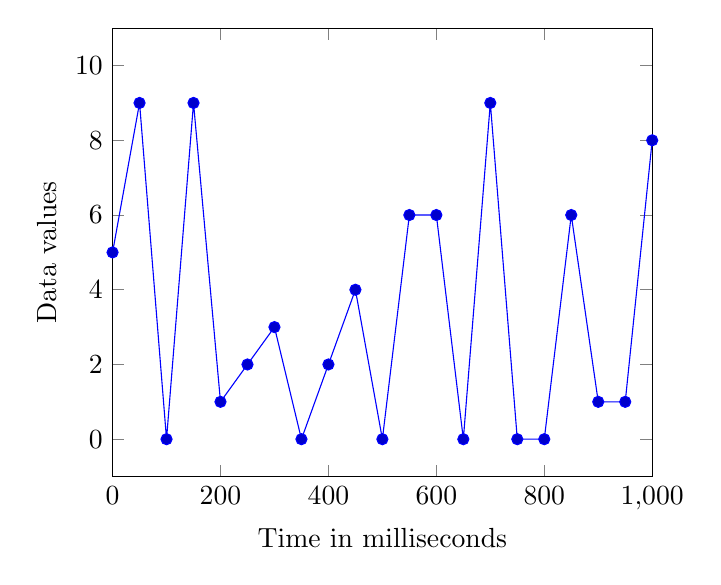
\begin{tikzpicture}
                    \begin{axis}[xmin=0, xmax=1000, ymin=-1, ymax=11, xlabel=Time in milliseconds, ylabel=Data values]
                        \addplot coordinates {
                            (0,5)
                            (50,9)
                            (100,0)
                            (150,9)
                            (200,1)
                            (250,2)
                            (300,3)
                            (350,0)
                            (400,2)
                            (450,4)
                            (500,0)
                            (550,6)
                            (600,6)
                            (650,0)
                            (700,9)
                            (750,0)
                            (800,0)
                            (850,6)
                            (900,1)
                            (950,1)
                            (1000,8)
                        };
                    \end{axis}
                \end{tikzpicture}
            } &
            \resizebox {0.25\textwidth} {!} {
                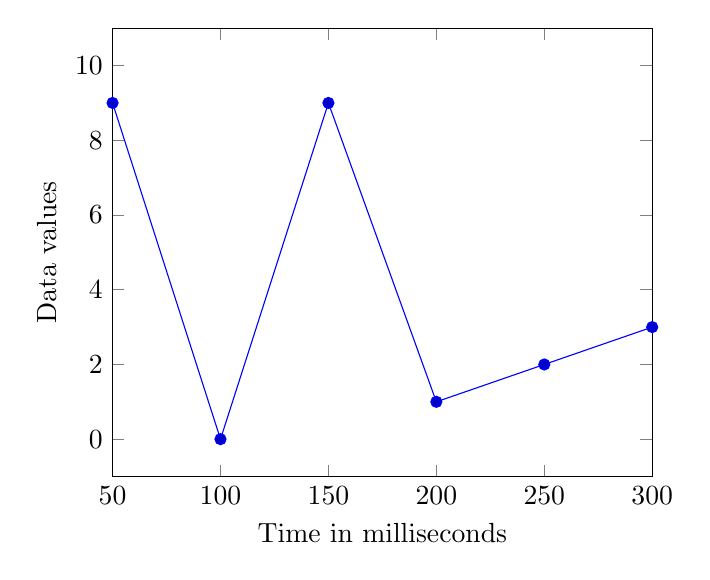
\begin{tikzpicture}
                    \begin{axis}[xmin=50, xmax=300, ymin=-1, ymax=11, xlabel=Time in milliseconds, ylabel=Data values]
                        \addplot coordinates {
                            (50,9)
                            (100,0)
                            (150,9)
                            (200,1)
                            (250,2)
                            (300,3)
                        };
                    \end{axis}
                \end{tikzpicture}
            } &
            \resizebox {0.25\textwidth} {!} {
                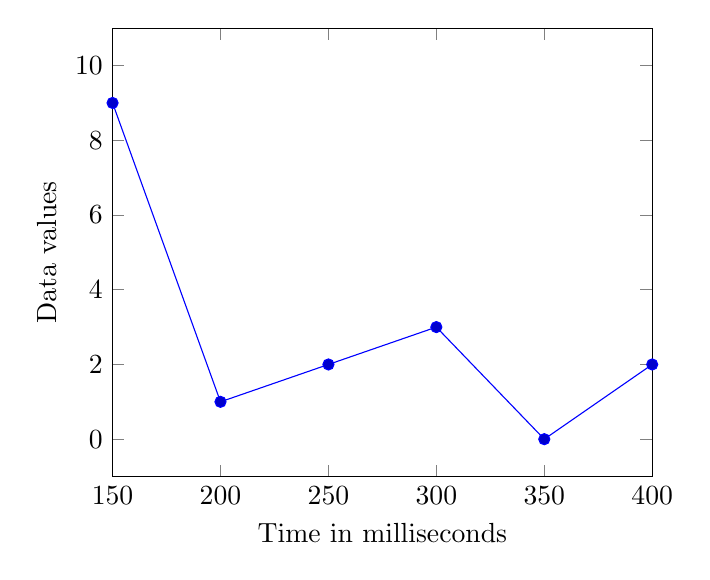
\begin{tikzpicture}
                    \begin{axis}[xmin=150, xmax=400, ymin=-1, ymax=11, xlabel=Time in milliseconds, ylabel=Data values]
                        \addplot coordinates {
                            (150,9)
                            (200,1)
                            (250,2)
                            (300,3)
                            (350,0)
                            (400,2)
                        };
                    \end{axis}
                \end{tikzpicture}
            } &
            \resizebox {0.25\textwidth} {!} {
                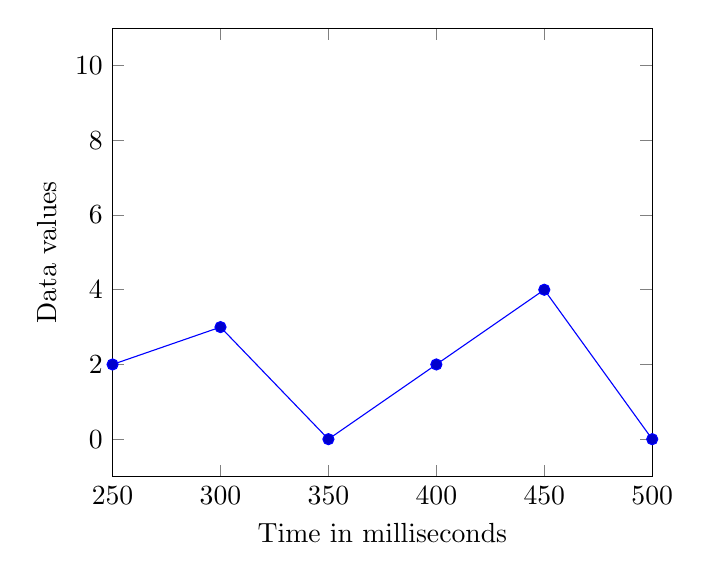
\begin{tikzpicture}
                    \begin{axis}[xmin=250, xmax=500, ymin=-1, ymax=11, xlabel=Time in milliseconds, ylabel=Data values]
                        \addplot coordinates {
                            (250,2)
                            (300,3)
                            (350,0)
                            (400,2)
                            (450,4)
                            (500,0)
                        };
                    \end{axis}
                \end{tikzpicture}
            } \\
            (a) & (b) & (c) & (d)
        \end{tabular}
        \caption{Data input example.}
        \label{fig:datainputgraph}
    \end{figure}

    A possible scenario is a software that gets every 100 milliseconds a time series interval or window like
    figure~\ref{fig:datainputgraph}(b) - (c) from a device. The software has to classify the time series window, for
    example with a one nearest neighbour algorithm and a distance measure like DTW. That way the software tries to guess
    a statement about the current situation of the device. Maybe the software has classifies the current window as a
    gesture that the holder of a smartwatch has performed.\\

    The combination of a one nearest neighbour algorithm with DTW as distance measure are a very common approach to
    classify time series. A more classic approach for a distance measure is the euclidean distance. The advantage is the
    linear time and space complexity, but the euclidean distance is brittle \cite{keogh2005exact} for time series that
    are out of phase in the time axis. Especially human made time series like gestures are often out of phase in the
    time axis.

    \section{Objectives}
    The approach of a sliding window filter for time series streams is to avoid unnecessary usage of the complex and
    time consuming DTW algorithm. The filter works as a bouncer in front of the one nearest neighbour classification
    with the DTW algorithm. The requirements for such a filter are linear time and space complexity.\\

    A very promising candidate for a fast filter is the complexity estimate from
    \textit{A Complexity-Invariant Distance Measure for Time Series} \cite{batista2011complexity}. The complexity
    estimate of a time series $Q$ with data points $q_1 \dots q_n$ can be calculated like this:\\
    \begin{center}
        $CE(Q) = \sqrt[2]{\sum \limits_{i=1}^{n-1} (q_i-q_{i+1})^2}$
    \end{center}

    An other promising candidate is the variance of a time series $Q$.\\
    \begin{center}
        $Var(Q) = \frac{1}{n -1} {\sum \limits_{i=1}^{n} (q_i-\bar{q}_n)^2}$ with
        $\bar{q}_n = \frac{1}{n} {\sum \limits_{i=1}^{n} q_i}$
    \end{center}

    Both candidates have linear time and space complexity. It is not excluded that other filters are tried out during
    the bachelor thesis.\\

    The precondition for a filter is knowledge about the measure of every time series in the training set.
    A simple approach for the filter would be to allow only time series windows for classification that have a
    measure between the lower and the upper bound of our training set.

    \section{Evaluation}
    The sliding window filter idea can possibly work in many domains. For example to detecting keywords in audio
    streams or detecting gestures in the acceleration data of a smartwatch. I will focus my research on the gesture
    detection inspired by
    \textit{uWave: Accelerometer-based personalized gesture recognition and its applications} \cite{liu2009uwave}.

    \subsection{Experiment}
    I have created a experiment to record the acceleration data from a Wii Remote controller that is used by a
    experimentee to perform gestures mixed with physical activity. A experimentee has to perform a number of tasks. The
    tasks are a mix of physical activity and performing gestures. Figure~\ref{fig:wii-remote} shows a Wii Remote Plus
    controller.

    \begin{figure}
        \centering
        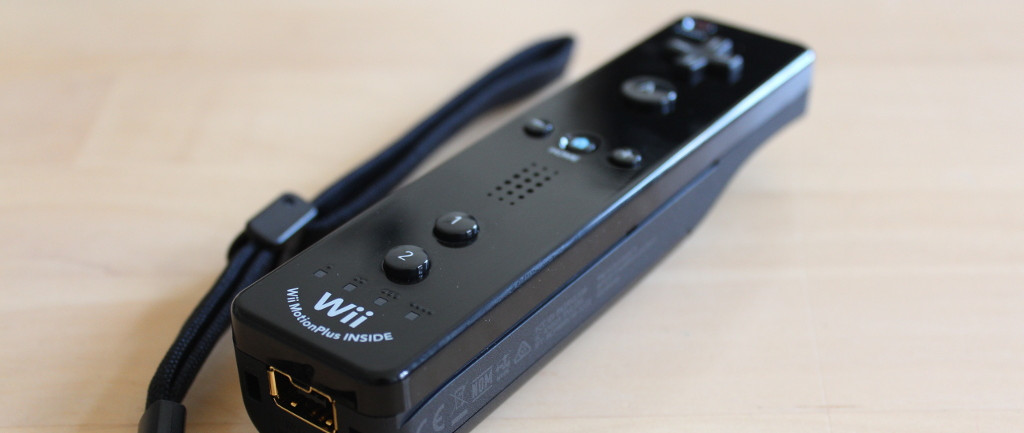
\includegraphics[width=0.9\textwidth]{wii-remote-plus.jpg}
        \caption{A black Wii Remote Plus controller.}
        \label{fig:wii-remote}
    \end{figure}

    \subsubsection{Implementation of the experiment}
    The program that is running the experiment is implemented in the programming language Python and available on
    GitHub\footnote{https://github.com/GordonLesti/SlidingWindowFilter-experiment}. The requirements to run the
    experiment are Python 2\footnote{https://www.python.org/}, xwiimote\footnote{https://github.com/dvdhrm/xwiimote} and
    xwiimote-bindings\footnote{https://github.com/dvdhrm/xwiimote-bindings}.

    \subsubsection{Course of the experiment}
    As mentioned above, one instance of the experiment will be performed with one experimentee and a Wii Remote
    controller. The tasks of the experiment will be communicated to the experimentee by a row of different screens that
    are changing after every gesture. Here are the rules of the experiment that will be explained to the experimentee
    before it begins.
    \begin{itemize}
        \item The Wii controller must be held in the same hand all the time during the hole experiment.
        \item The \textit{B} button of the controller is the trigger on the bottom of the controller.
        \item A gesture has to be performed by pressing the \textit{B} button down, holding the button, performing the
        gesture simultaneously and releasing the button after the gesture.
        \item It is not allowed to push the \textit{B} button outside of a gesture that is demanded by the experiment.
    \end{itemize}

    \paragraph{Task screens} are just images that are changing like a presentation after every gesture performed by the
    experimentee. The screens are shown in figure~\ref{fig:screens} and have the following functions.
    \begin{itemize}
        \item Screen \textit{(a)} is just welcoming the experimentee.
        \item Screen \textit{(b)} to \textit{(i)} are only for training gestures recordings.
        \item Screen \textit{(j)} to \textit{(q)} containing a physical activity followed by a gesture.
        \item Screen \textit{(r)} is just thanking the experimentee.
        \item Screen \textit{(s)} is just closing the experiment.
    \end{itemize}
    The program that is running during the experiment is recording the acceleration data from the Wii Remote controller
    all the time. Also the button down event of the \textit{B} button and the button up event will be recorded. The
    program will switch to the next task screen after every button up event, means after every gesture.

    \begin{figure}
        \centering
        \begin{tabular}{ccc}
            \frame{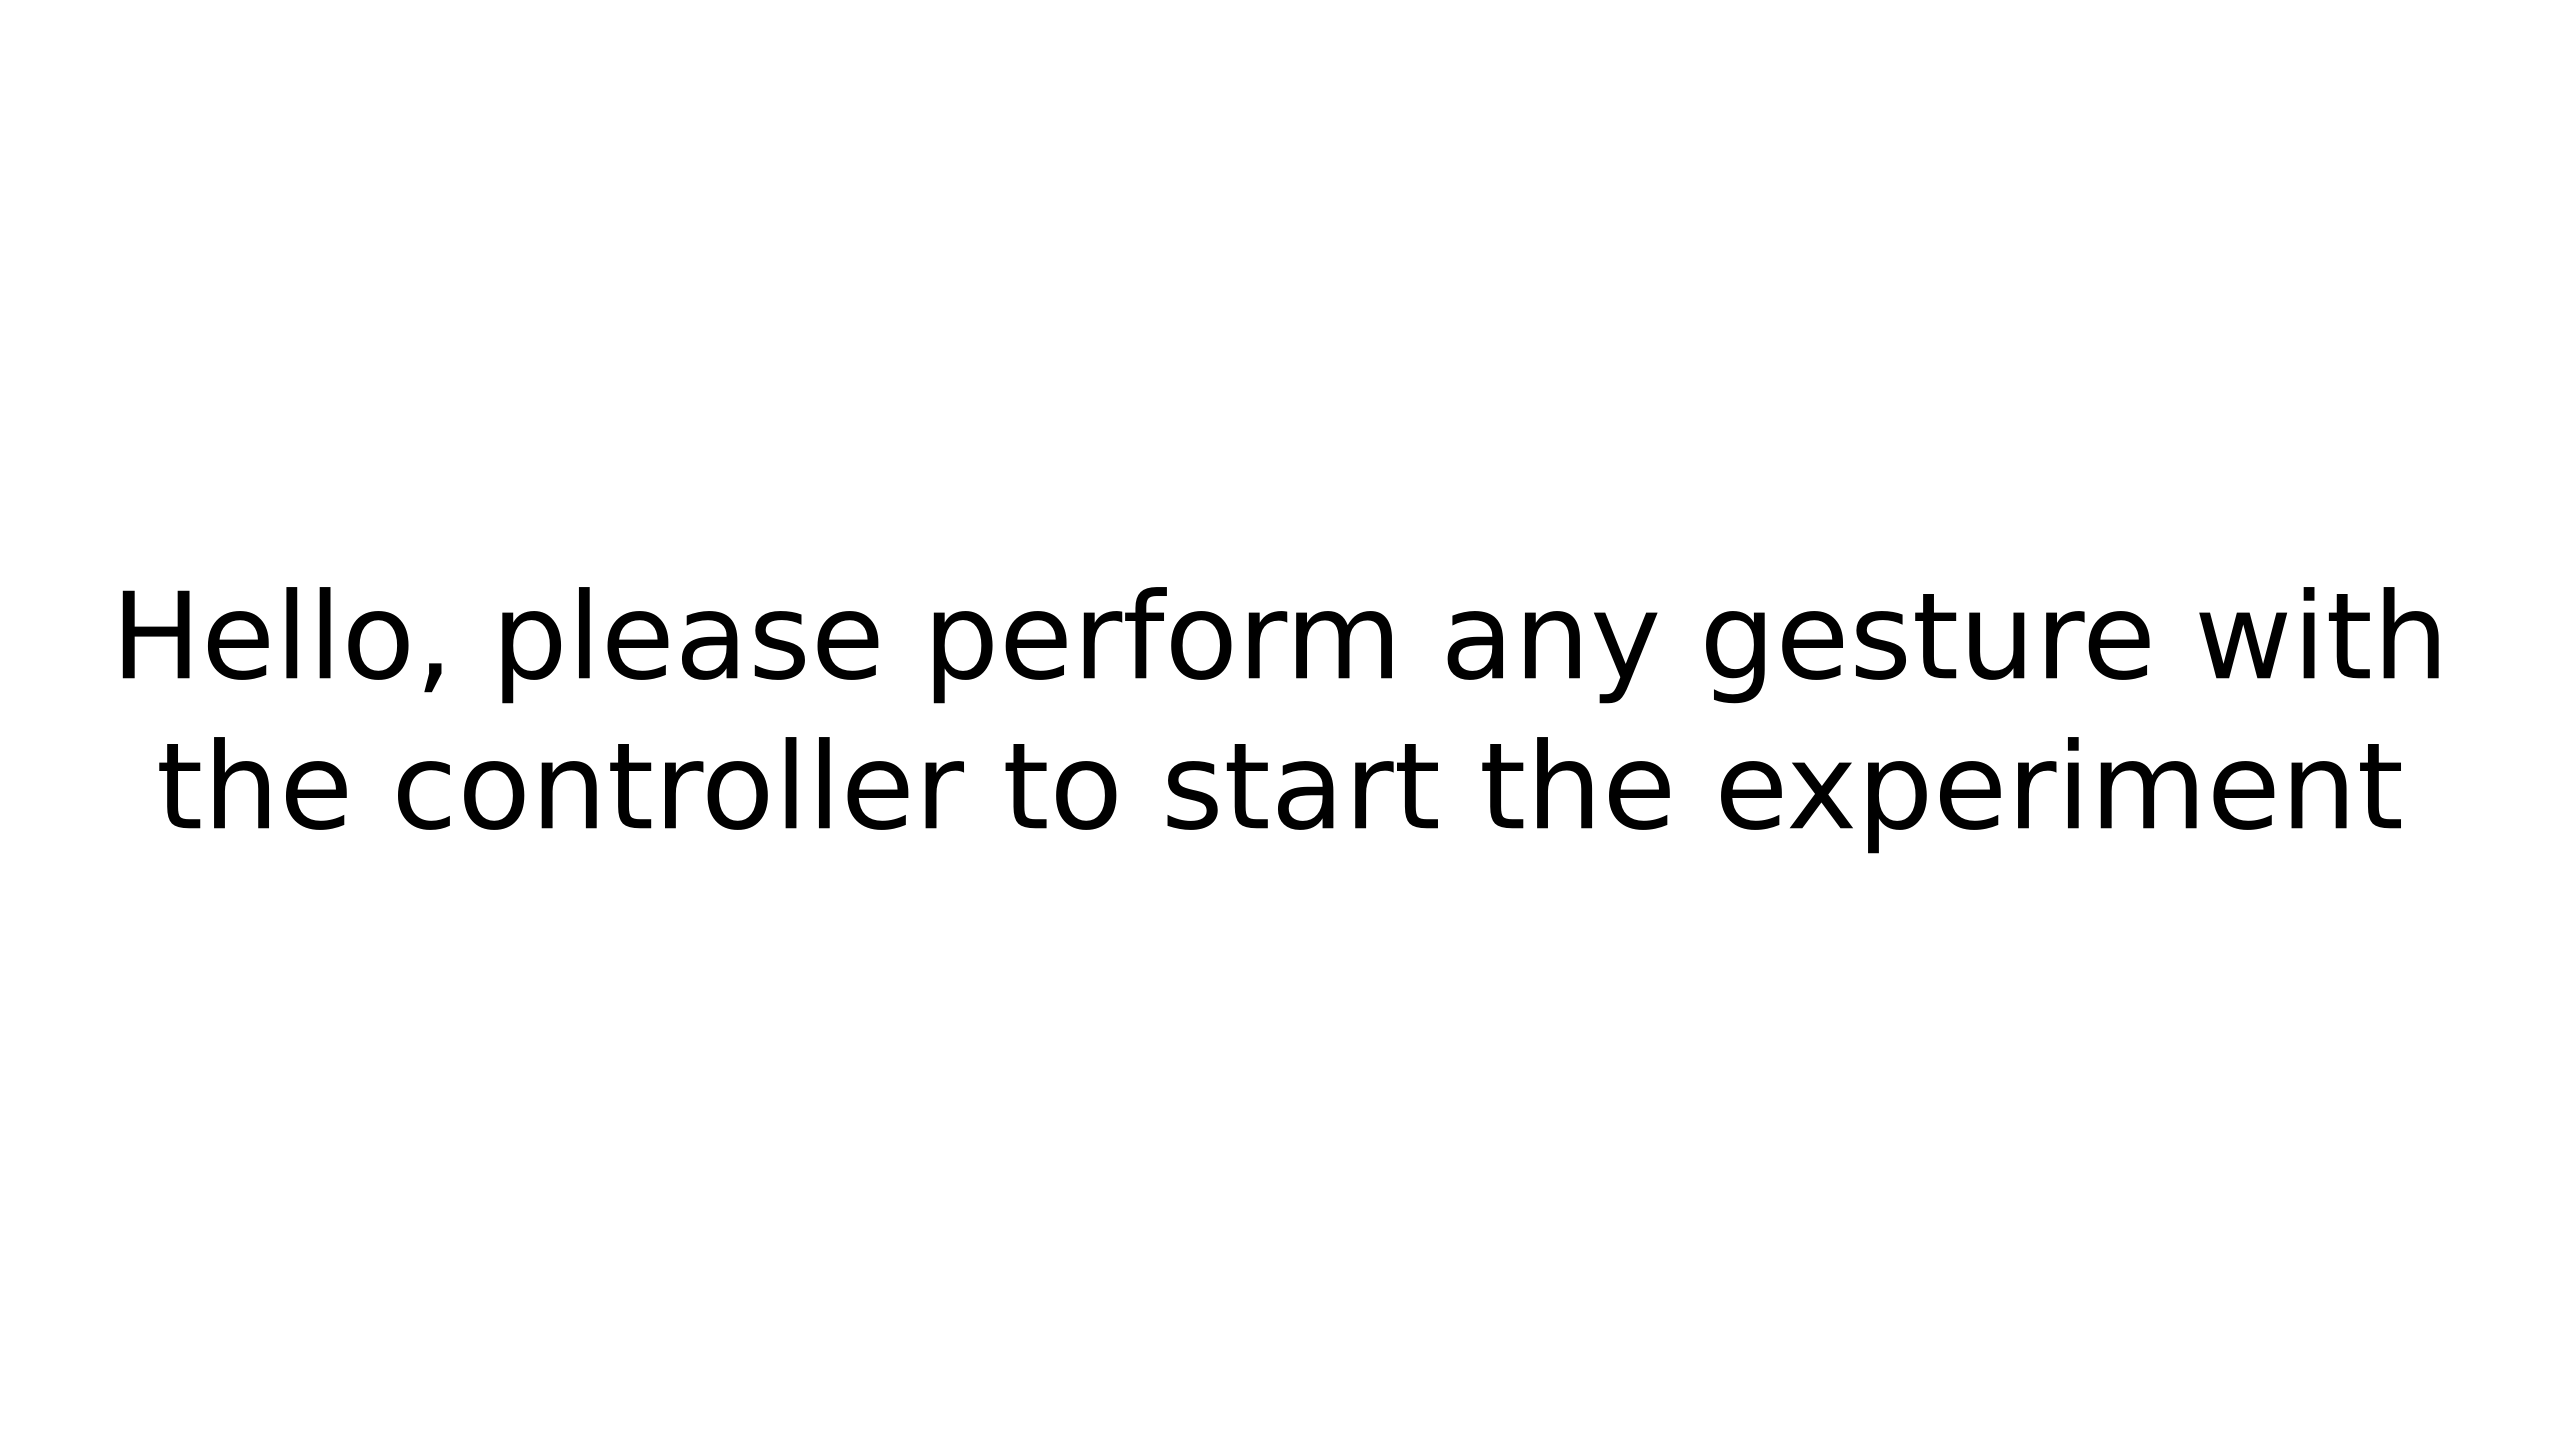
\includegraphics[width=0.3\textwidth]{1.png}} & \frame{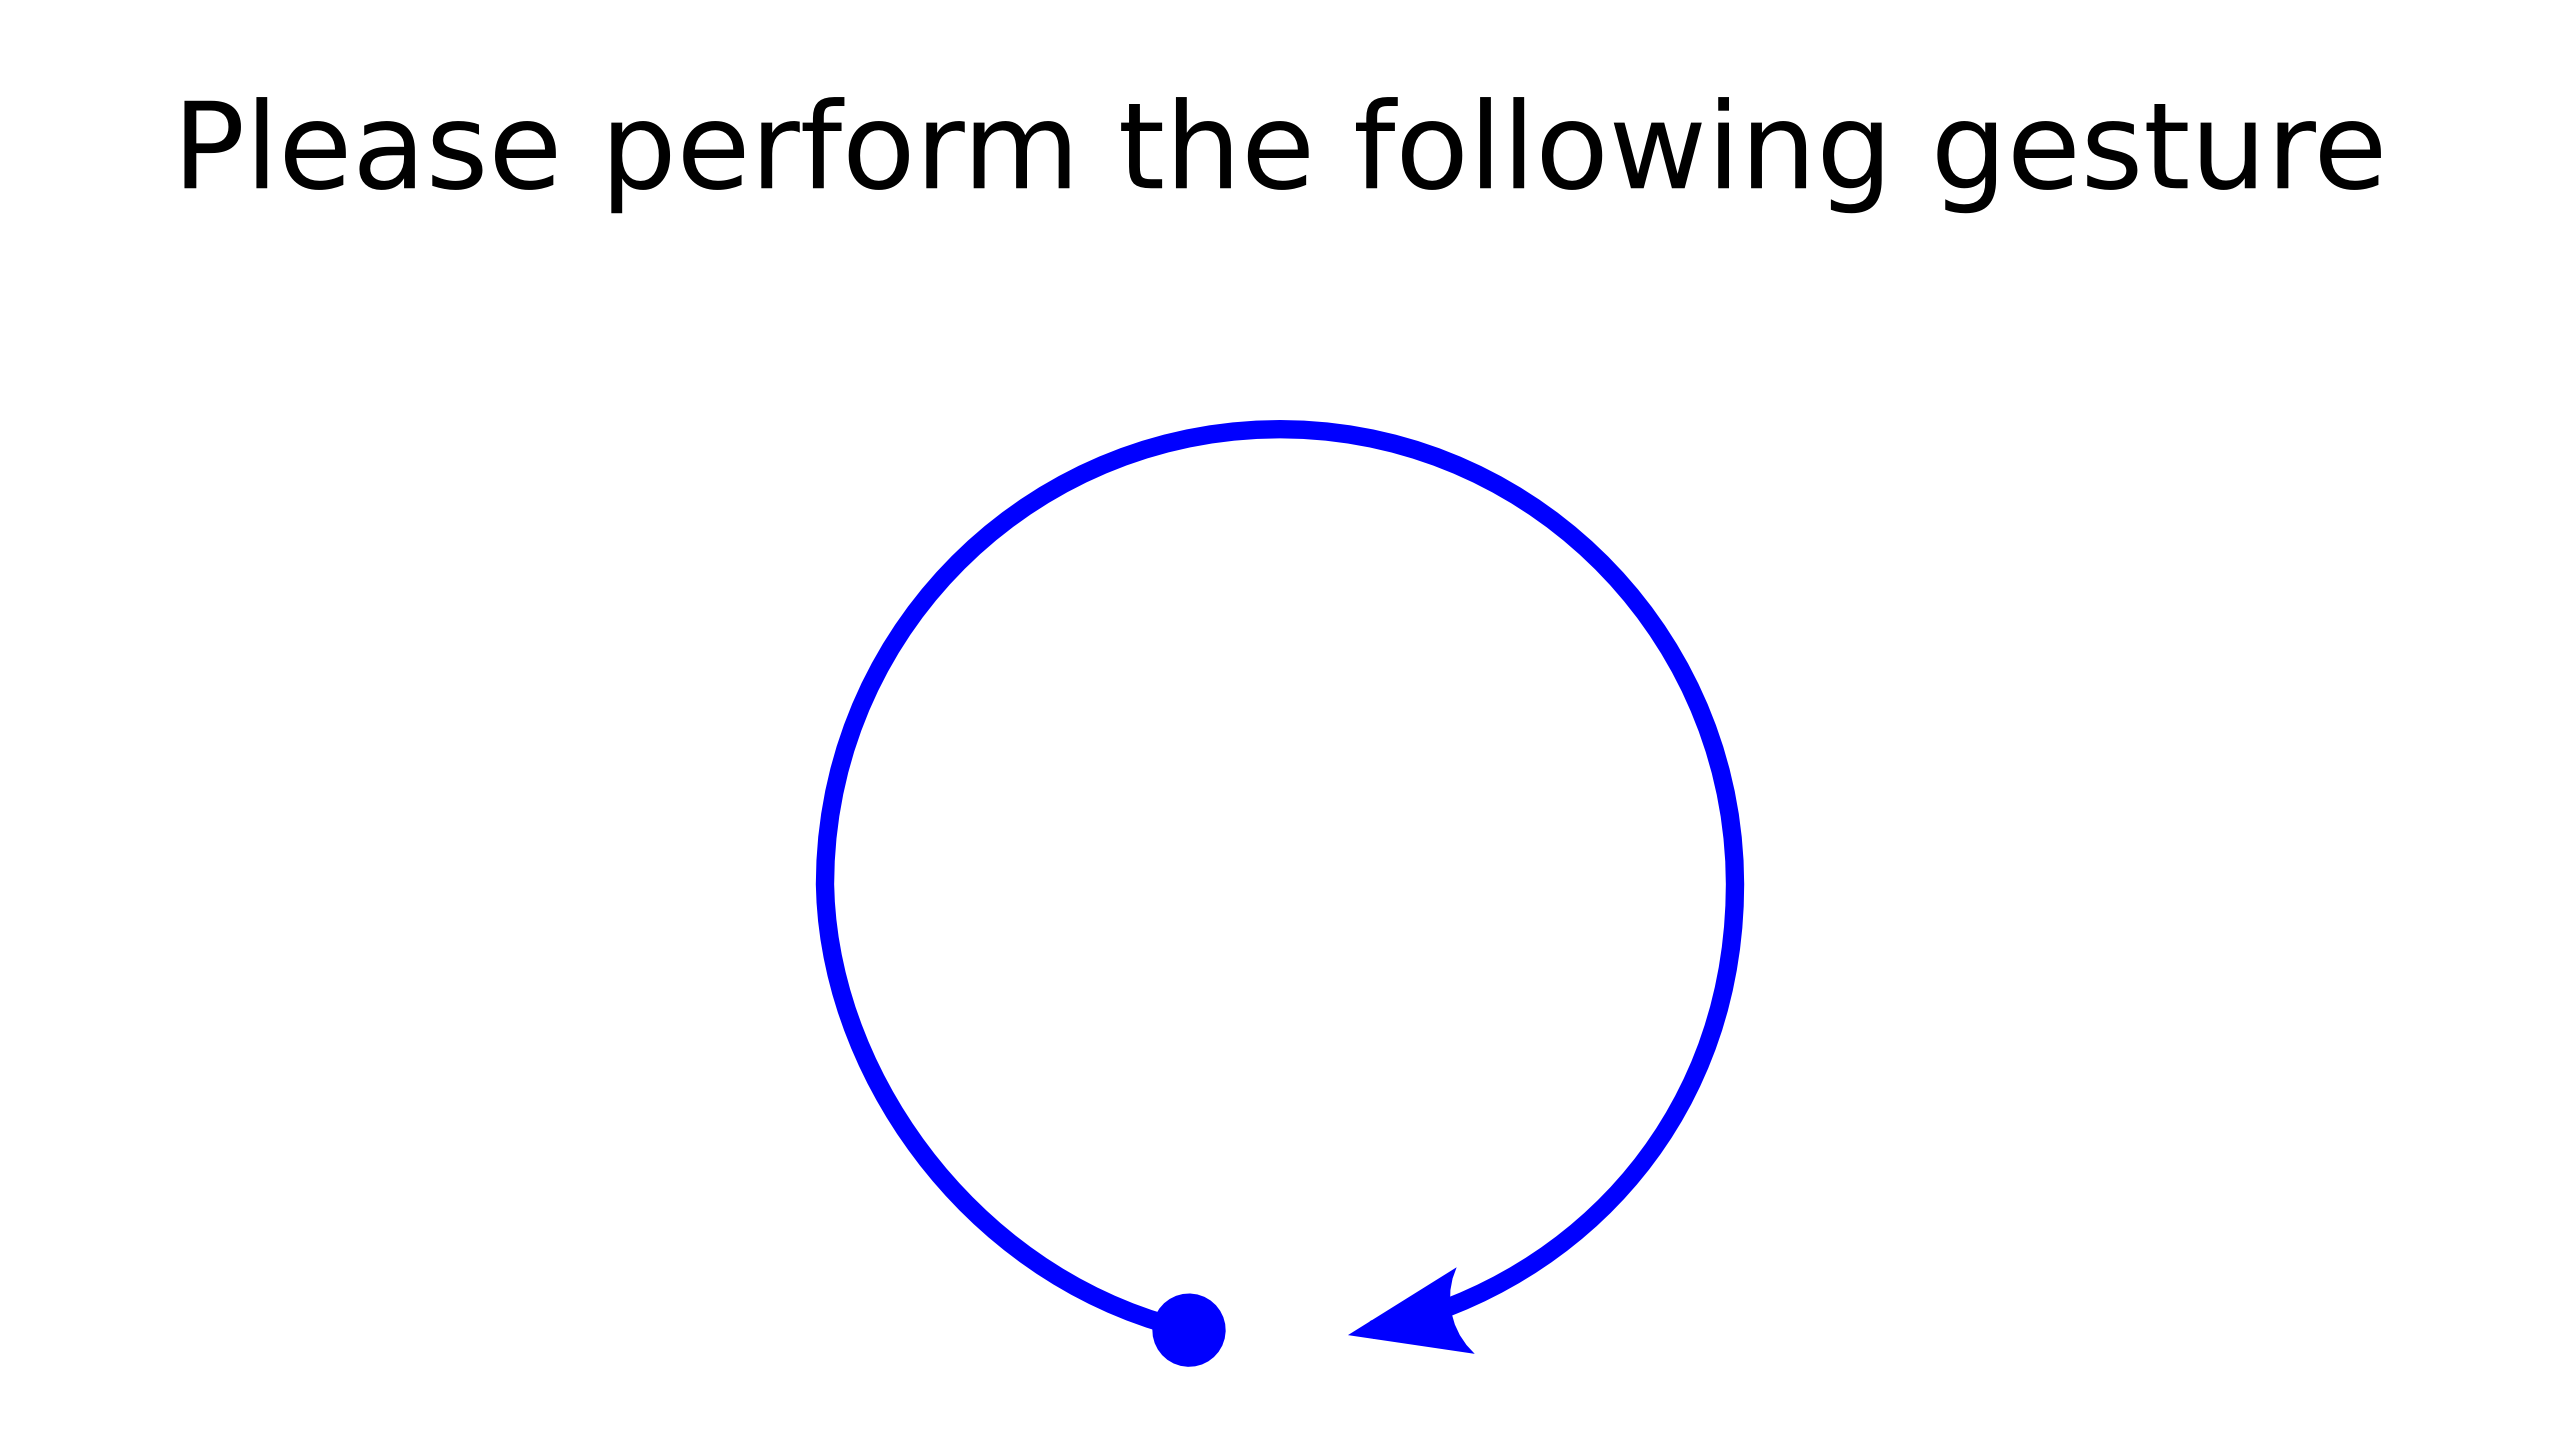
\includegraphics[width=0.3\textwidth]{2.png}} & \frame{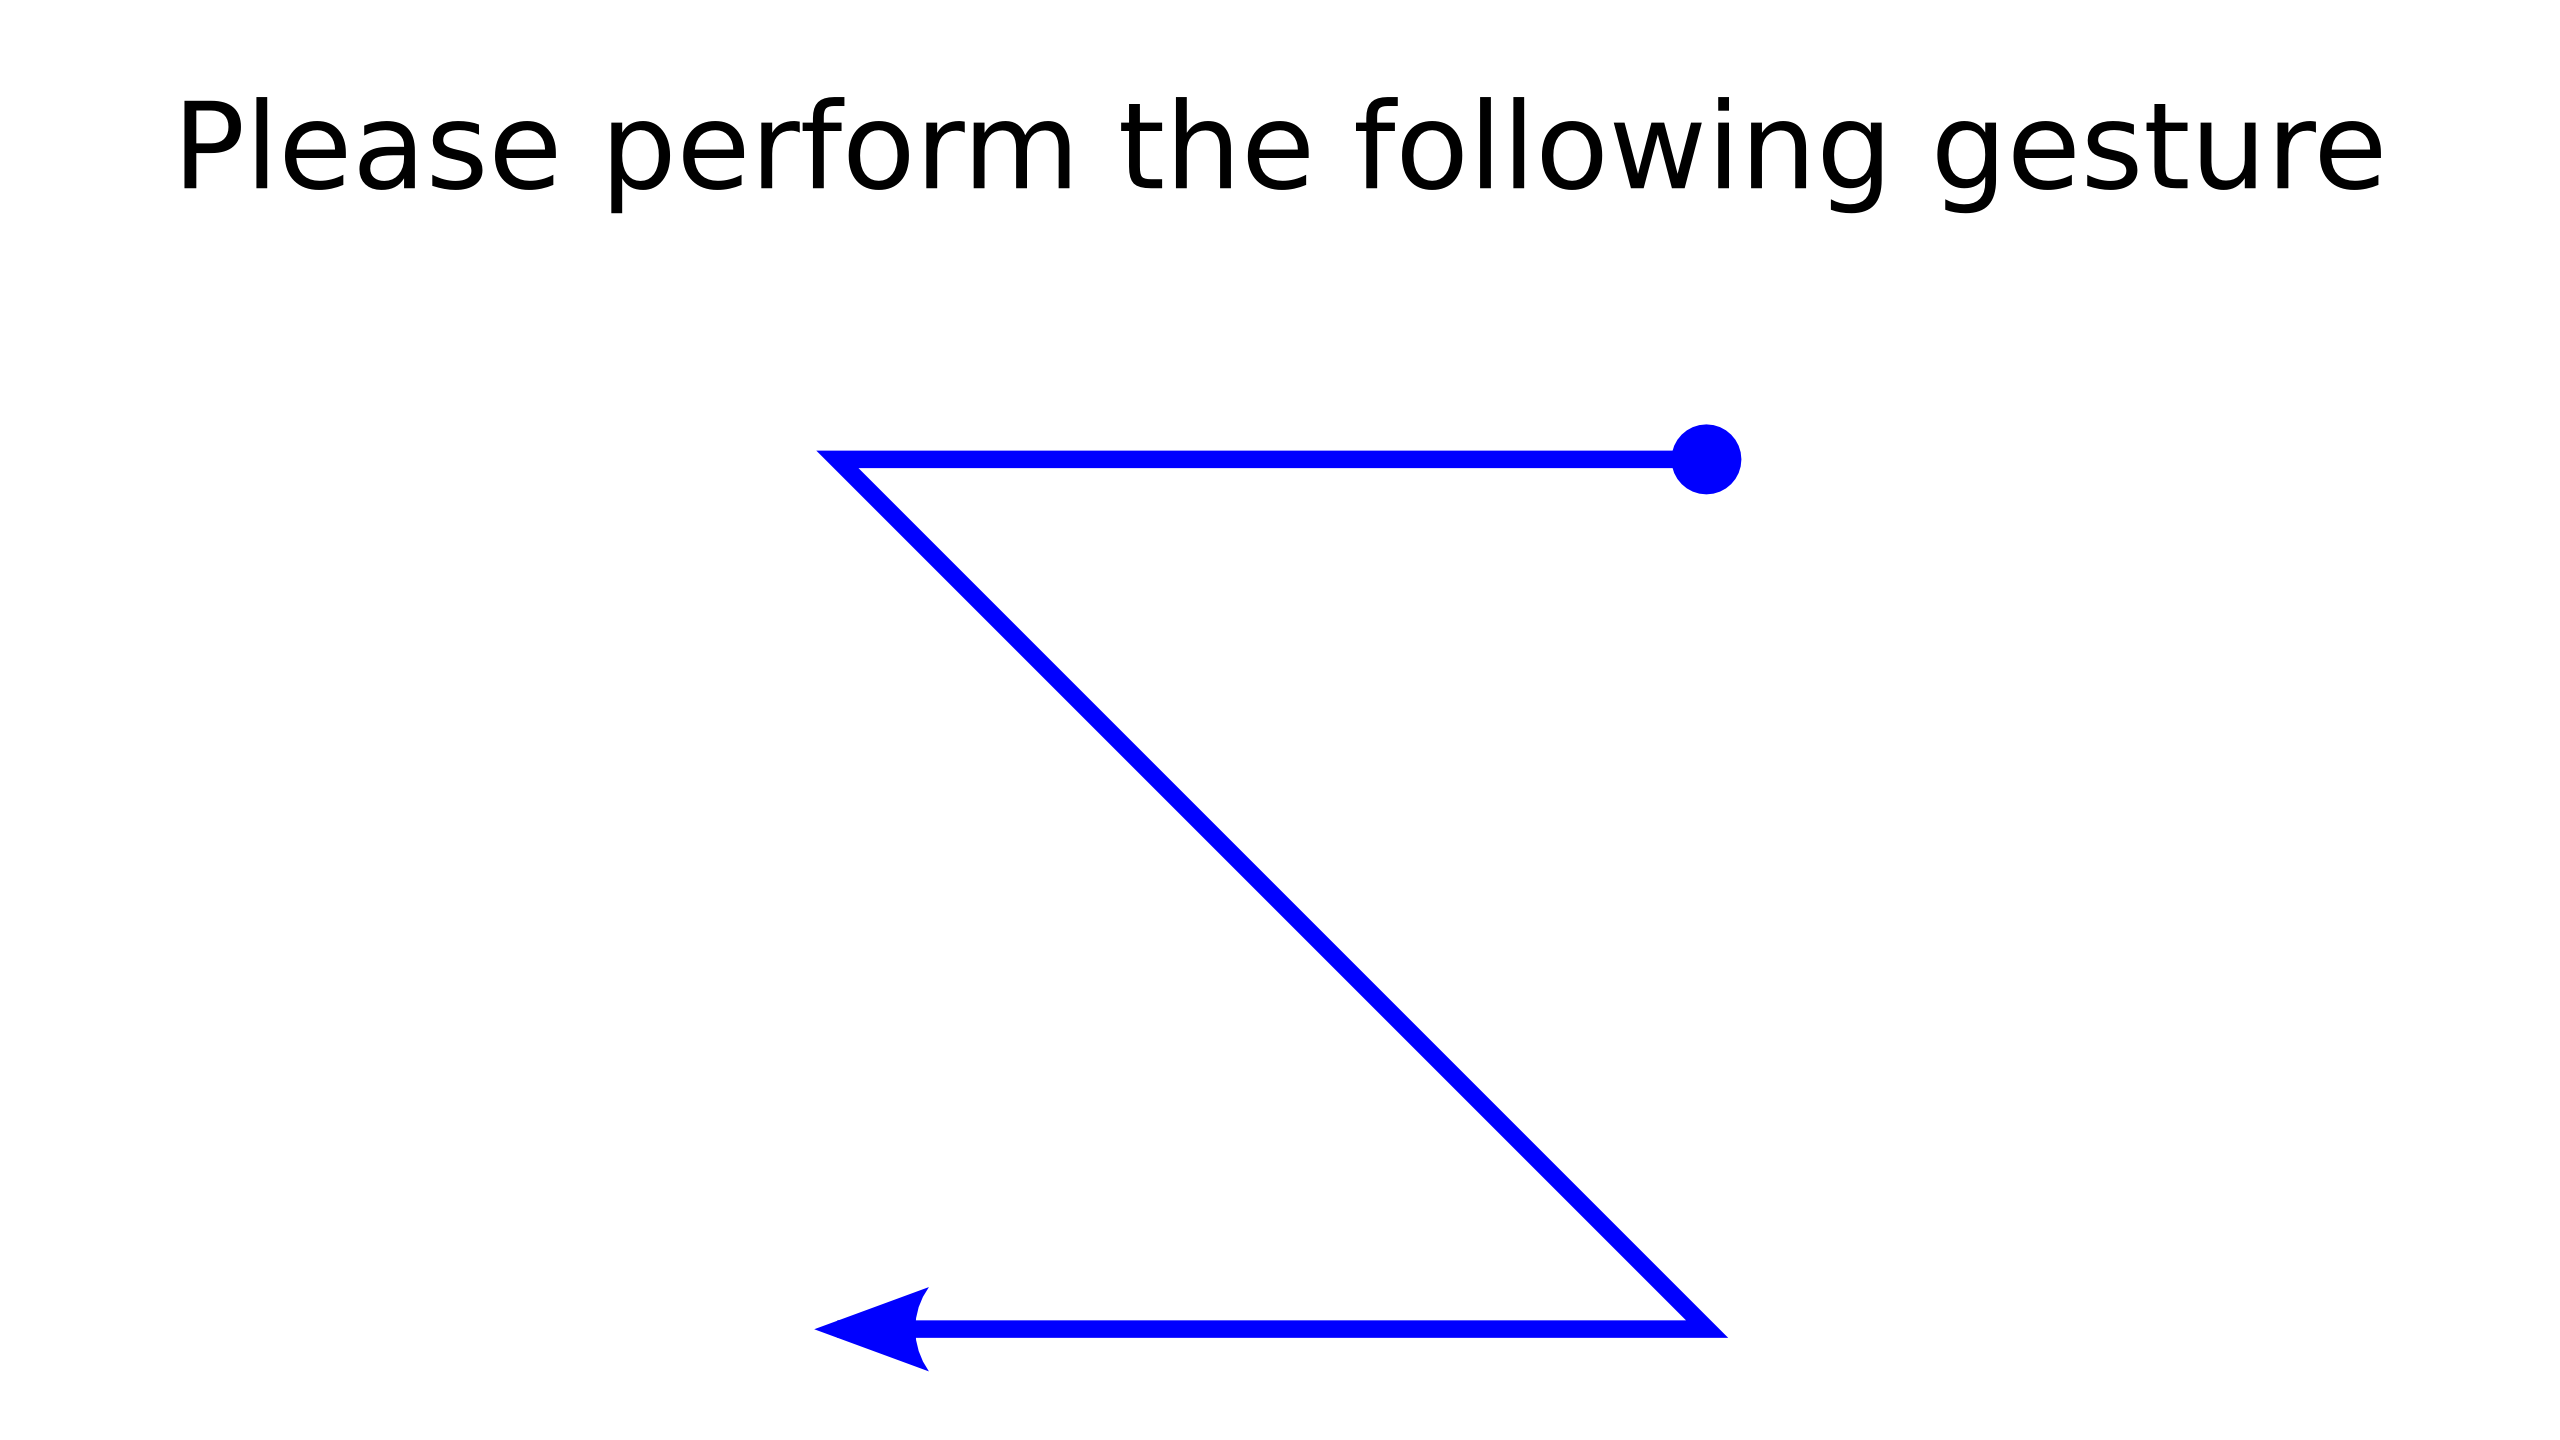
\includegraphics[width=0.3\textwidth]{3.png}} \\
            (a) \vspace{0.5ex} & (b) \vspace{0.5ex} & (c) \vspace{0.5ex} \\
            \frame{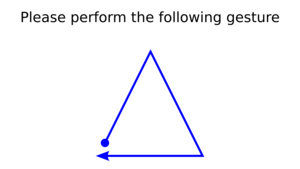
\includegraphics[width=0.3\textwidth]{4.png}} & \frame{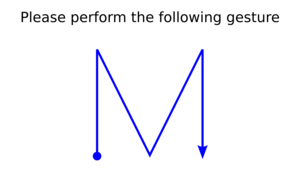
\includegraphics[width=0.3\textwidth]{5.png}} & \frame{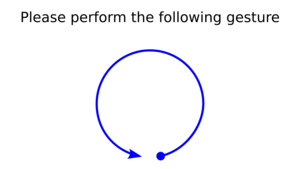
\includegraphics[width=0.3\textwidth]{6.png}} \\
            (d) \vspace{0.5ex} & (e) \vspace{0.5ex} & (f) \vspace{0.5ex} \\
            \frame{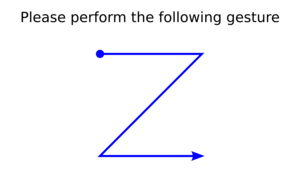
\includegraphics[width=0.3\textwidth]{7.png}} & \frame{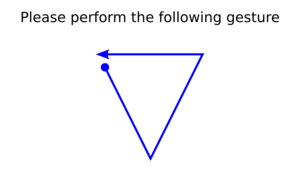
\includegraphics[width=0.3\textwidth]{8.png}} & \frame{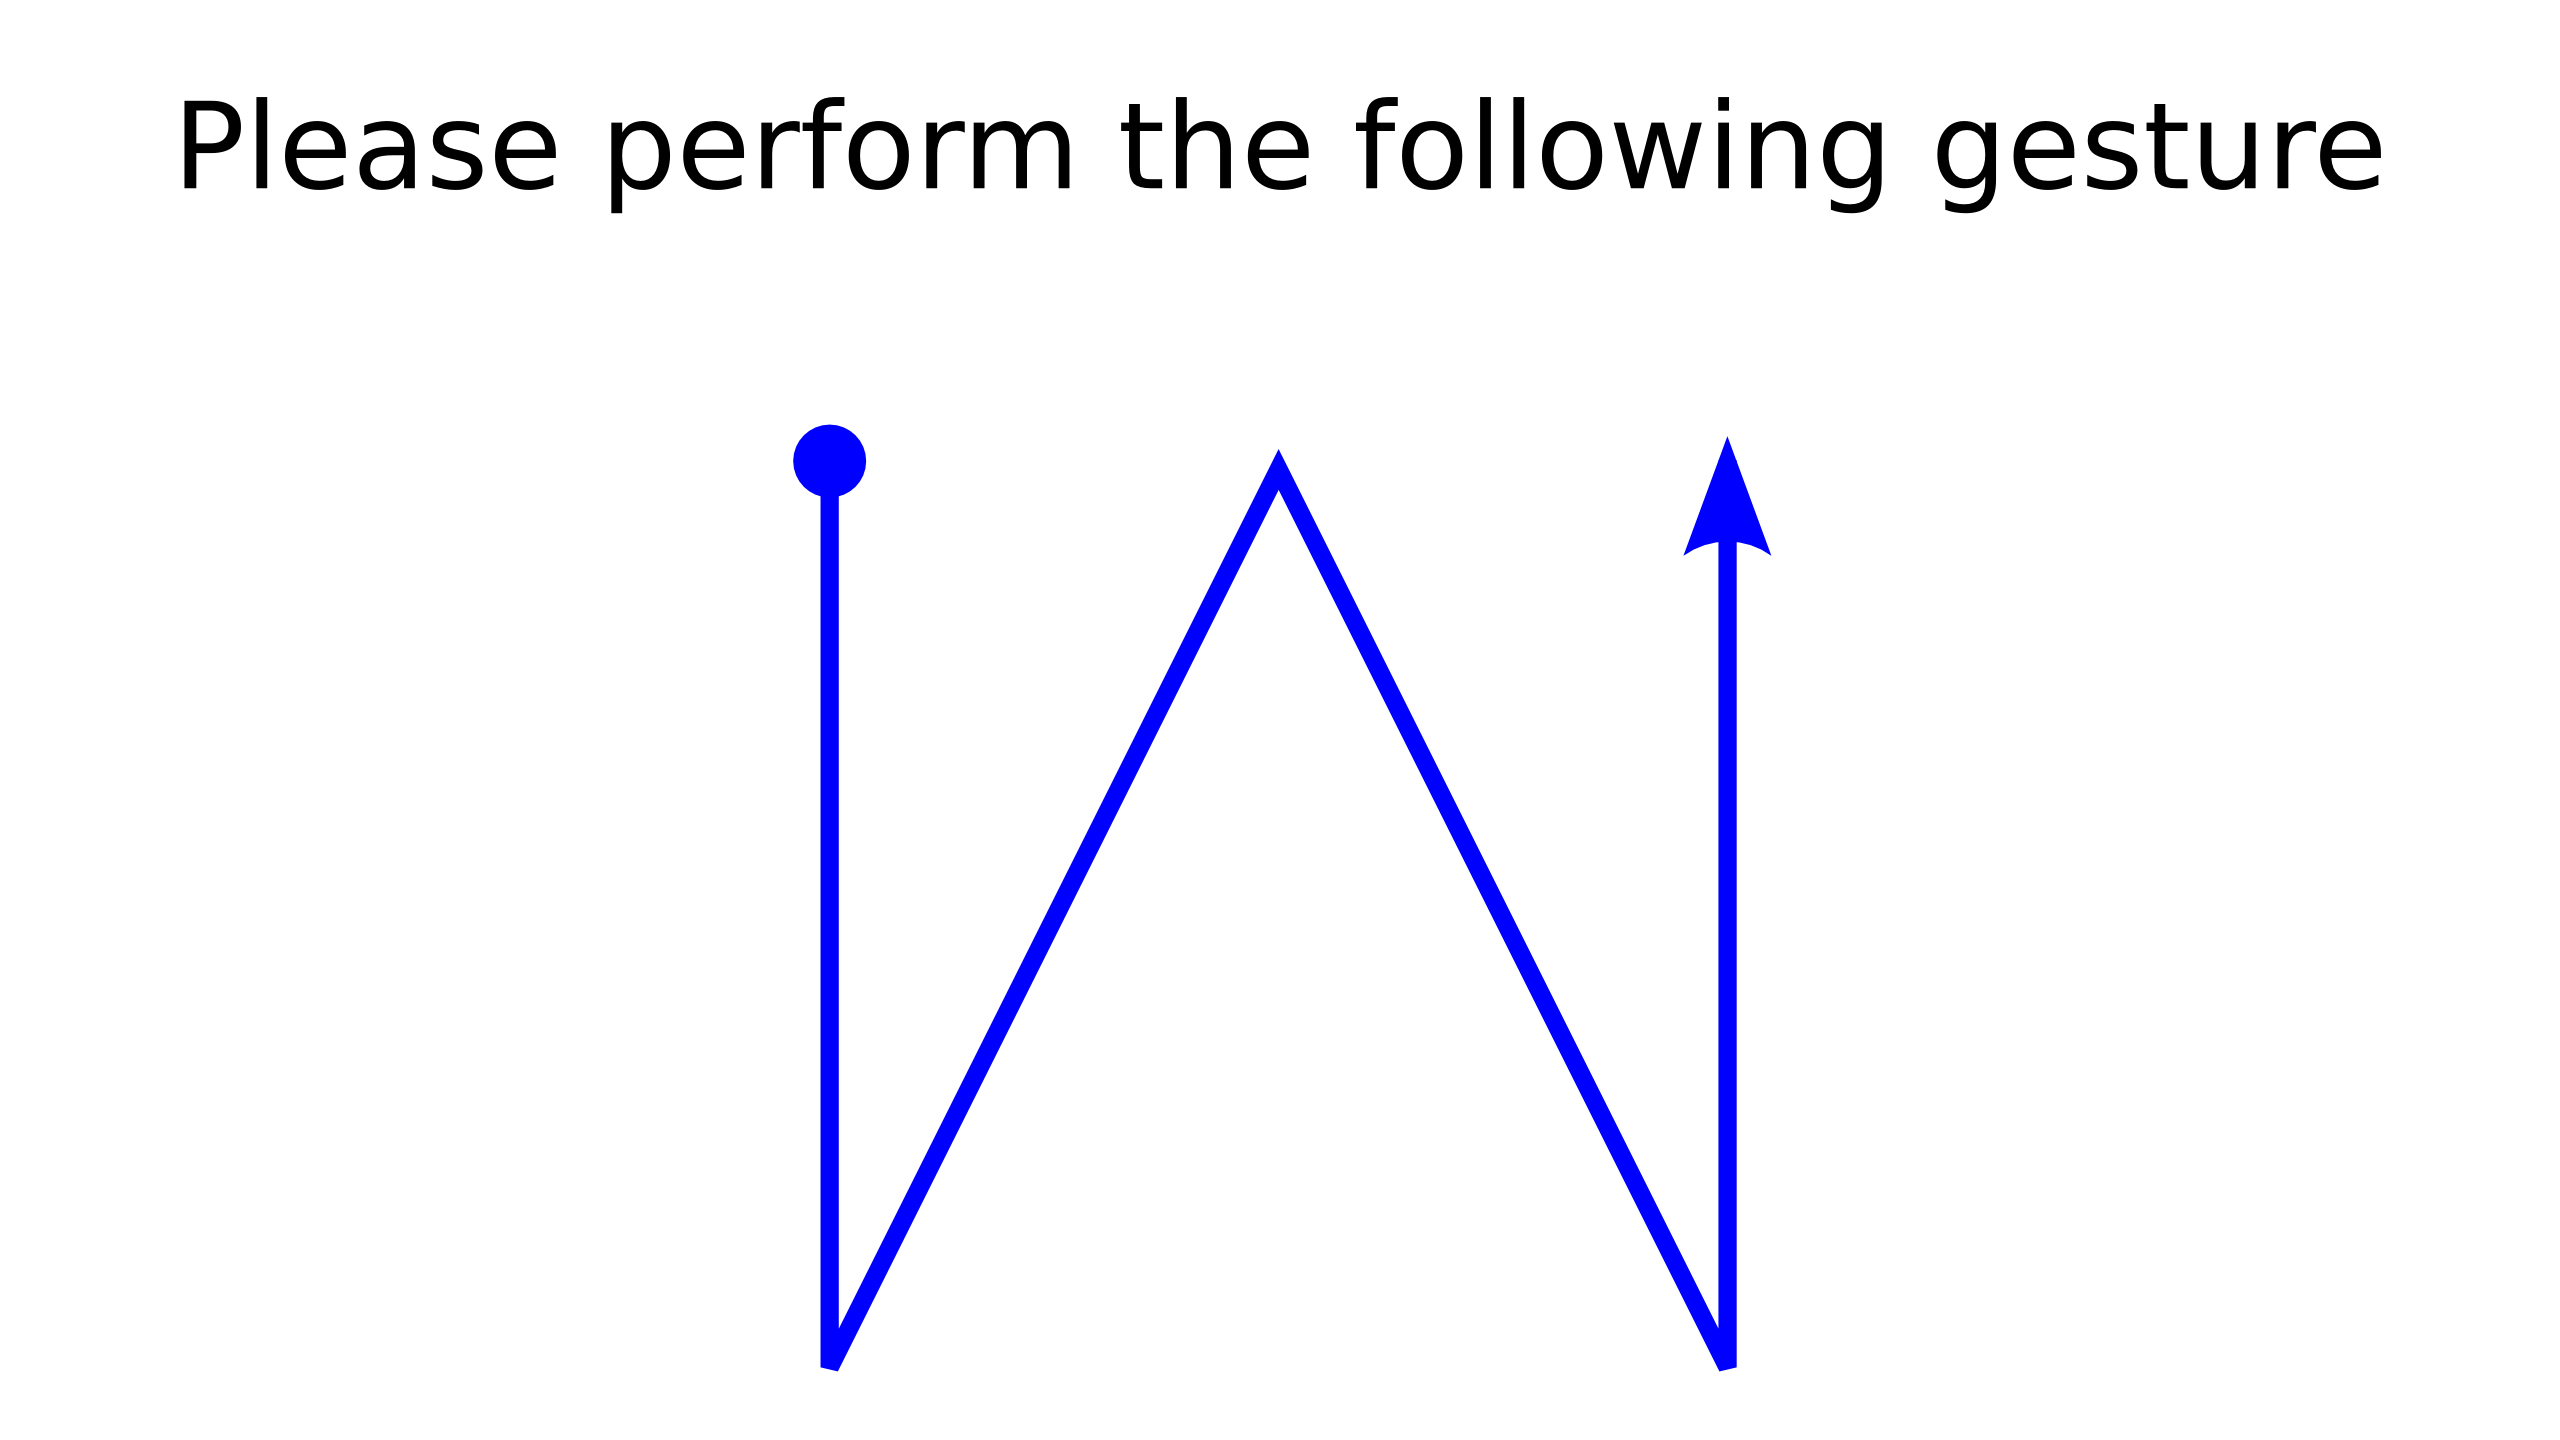
\includegraphics[width=0.3\textwidth]{9.png}} \\
            (g) \vspace{0.5ex} & (h) \vspace{0.5ex} & (i) \vspace{0.5ex} \\
            \frame{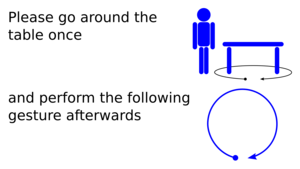
\includegraphics[width=0.3\textwidth]{10.png}} & \frame{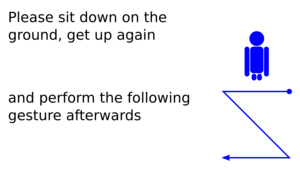
\includegraphics[width=0.3\textwidth]{11.png}} & \frame{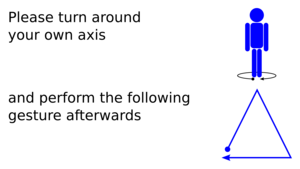
\includegraphics[width=0.3\textwidth]{12.png}} \\
            (j) \vspace{0.5ex} & (k) \vspace{0.5ex} & (l) \vspace{0.5ex} \\
            \frame{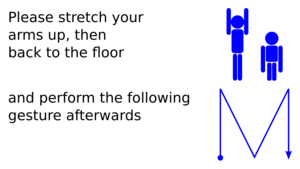
\includegraphics[width=0.3\textwidth]{13.png}} & \frame{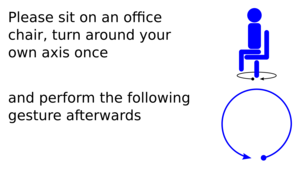
\includegraphics[width=0.3\textwidth]{14.png}} & \frame{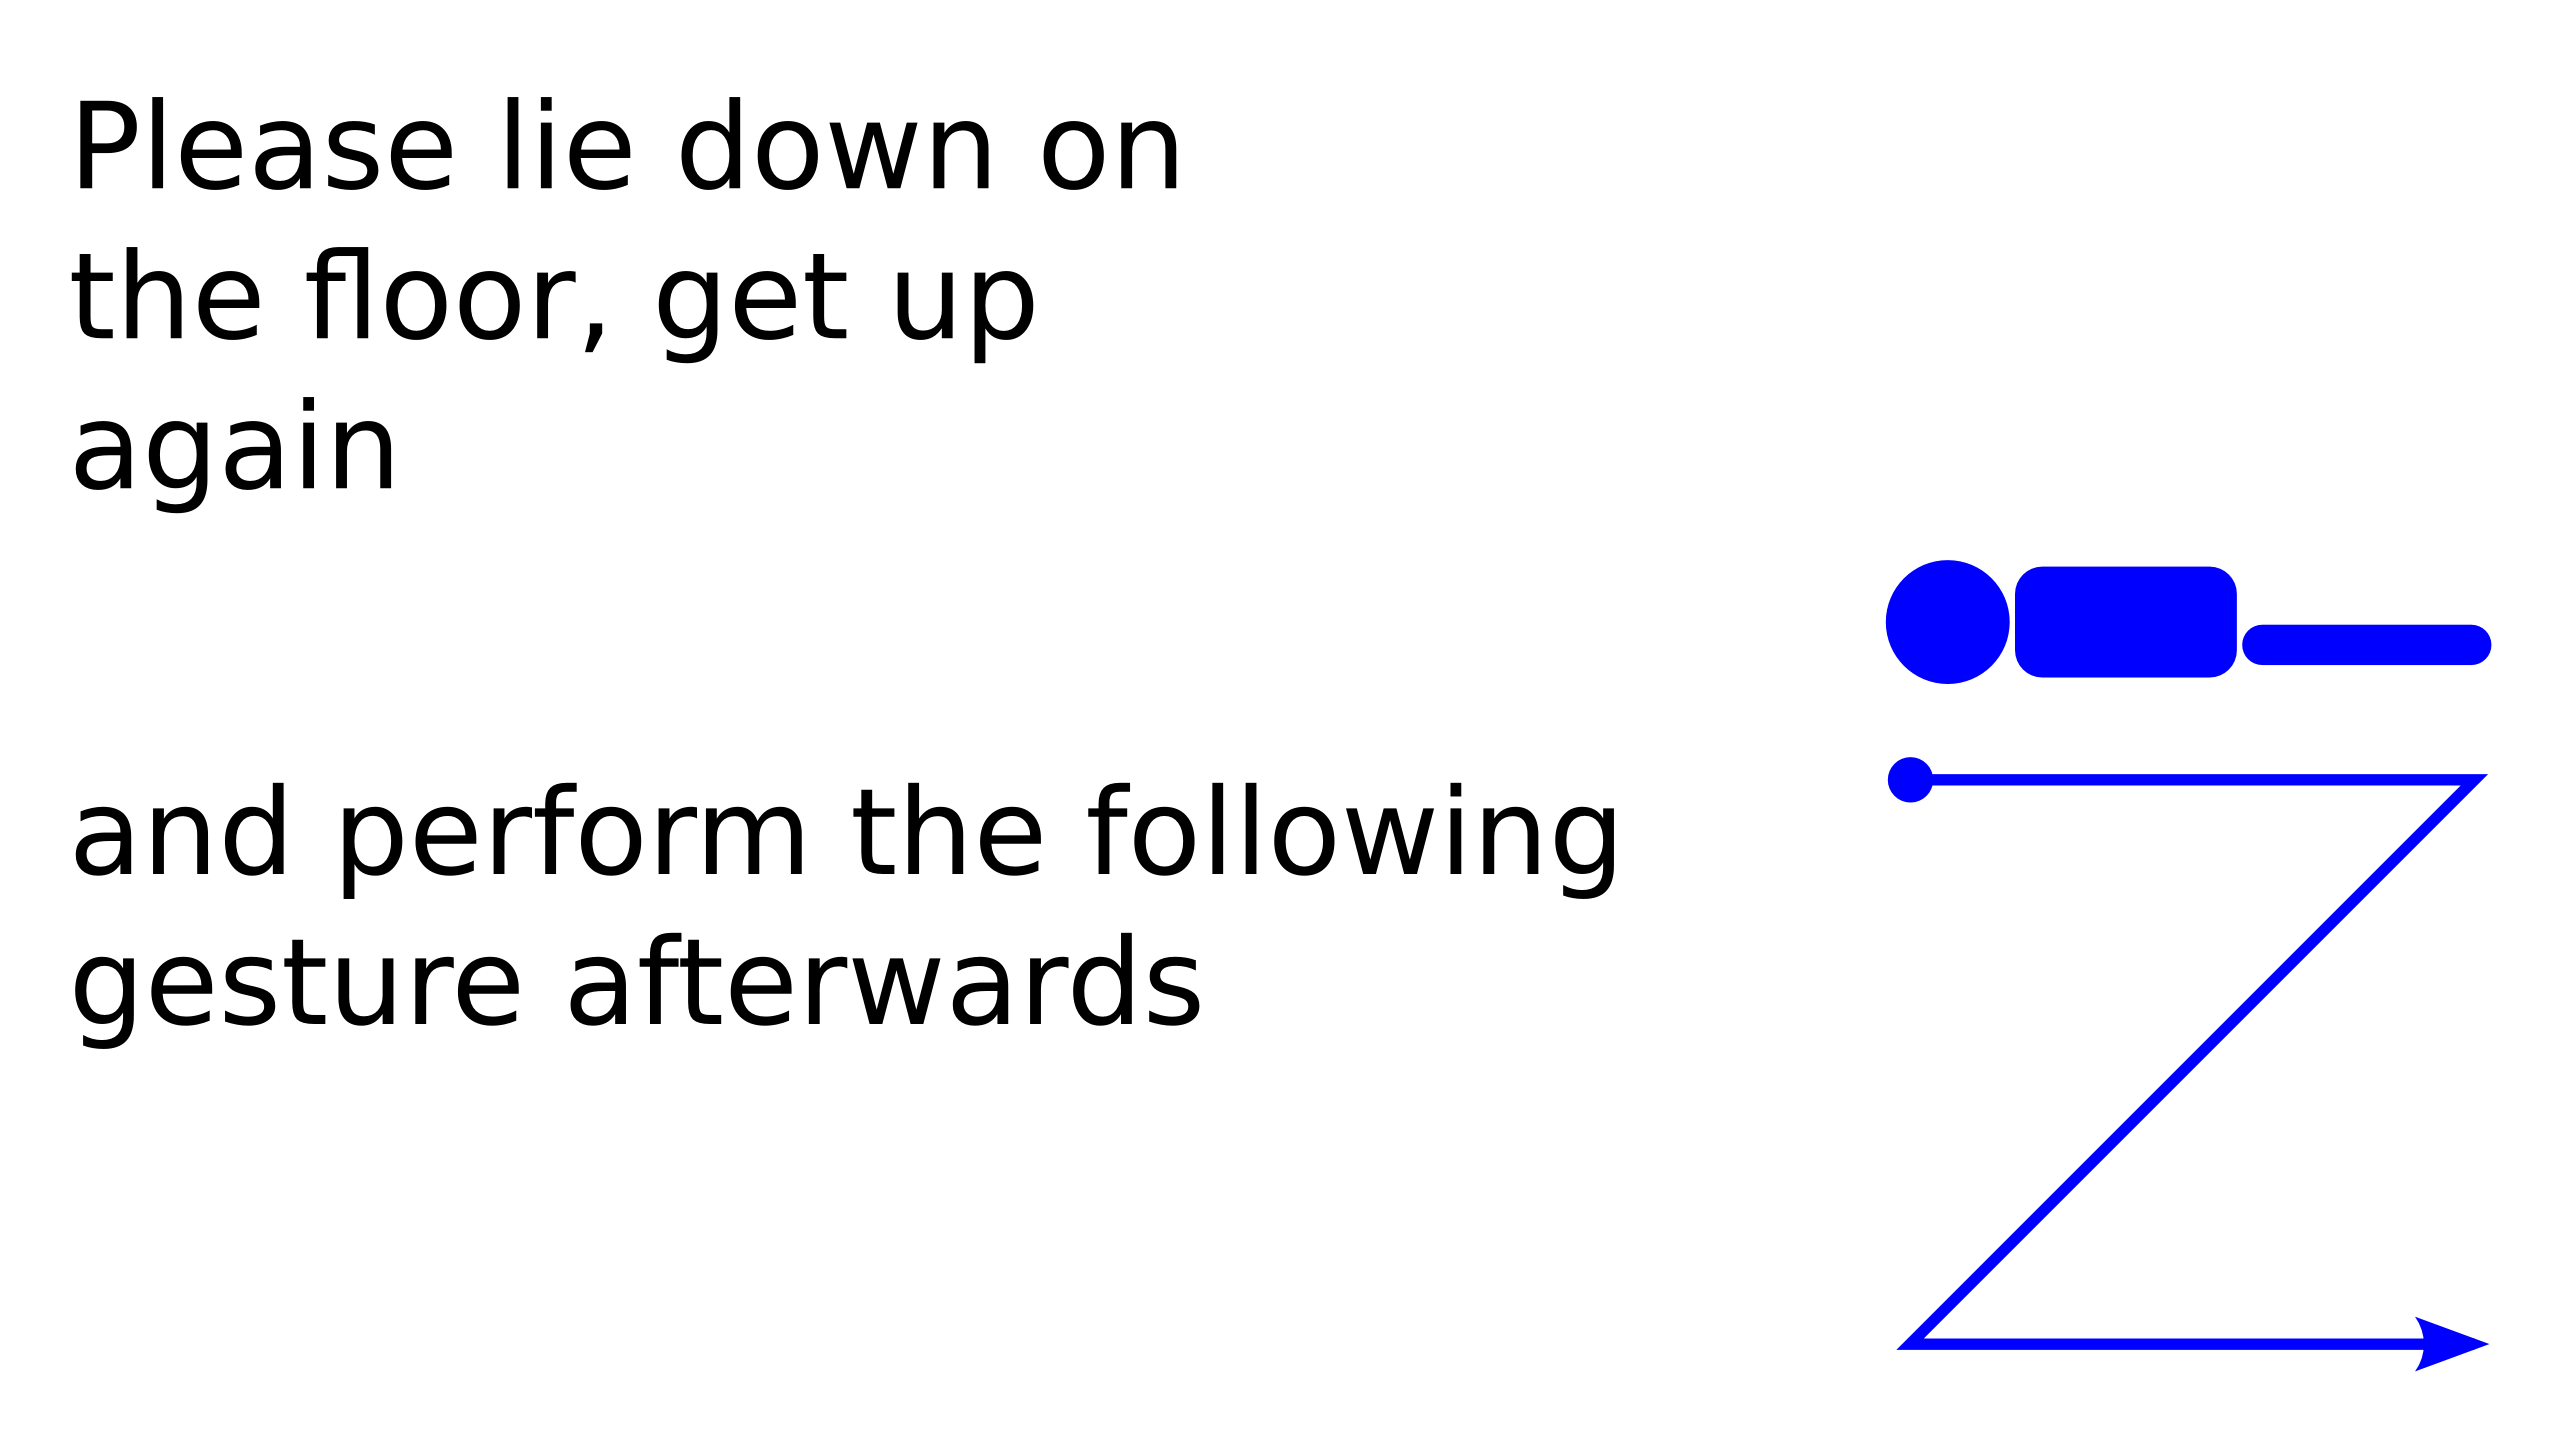
\includegraphics[width=0.3\textwidth]{15.png}} \\
            (m) \vspace{0.5ex} & (n) \vspace{0.5ex} & (o) \vspace{0.5ex} \\
            \frame{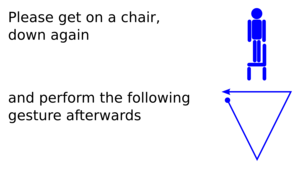
\includegraphics[width=0.3\textwidth]{16.png}} & \frame{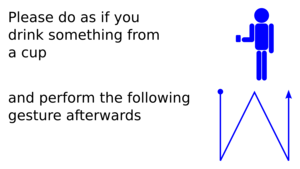
\includegraphics[width=0.3\textwidth]{17.png}} & \frame{
\includegraphics[width=0.3\textwidth]{18.png}} \\
            (p) \vspace{0.5ex} & (q) \vspace{0.5ex} & (r) \vspace{0.5ex} \\
            \multicolumn{3}{c}{\frame{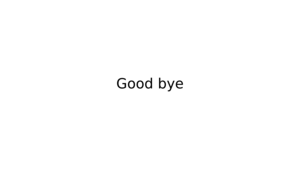
\includegraphics[width=0.3\textwidth]{19.png}}}\\
            \multicolumn{3}{c}{(s) \vspace{0.5ex}}\\
        \end{tabular}
        \caption{The task screens that will guide the experimentee.}
        \label{fig:screens}
    \end{figure}

    \subsubsection{Data from the experiment}

    The data of an experiment instance is always a file that contains lines of acceleration data and lines of button
    events. Every line will start with the count of milliseconds that have passed since the starting of the experiment.

    \paragraph{Acceleration data} lines contain the count of milliseconds that have passed since the starting of
    the experiment, the \textit{X} value, the \textit{Y} value and the \textit{Z} value of the acceleration data. Here
    an example for a acceleration data line.\\\\
    \verb+33085 -26 -6 89+

    \paragraph{Button down event} lines also contain the count of milliseconds that have passed since the starting
    of the experiment, the keyword \verb+START+ and the index of the gesture in the experiment starting with zero. Here
    an example for a button down event line.\\\\
    \verb+34315 START 4+

    \paragraph{Button up event} lines also contain the count of milliseconds that have passed since the starting
    of the experiment, the keyword \verb+END+ and the index of the gesture in the experiment starting with zero. Here
    an example for a button up event line.\\\\
    \verb+36375 END 4+\\

    The experiment contains nineteen screens and the program is recording from showing the first screen to showing the
    last screen. That means the resulting file will contain eighteen gesture start and end events.

    % Experiementeller Aufbau beschreiben

    %%% SPÄTER
    % Resultate aufzeigen
    % Diskusion mit eigener Interpretation

    % Conclusion
    %% Zukünftiges
    % Future Work
    % References

    \begin{thebibliography}{1}
        \bibitem{berndt1994using} Berndt, Donald J and Clifford, James "Using Dynamic Time Warping to Find Patterns in
        Time Series." KDD workshop (1994): 359--370
        \bibitem{keogh2005exact} Keogh, Eamonn and Ratanamahatana, Chotirat Ann "Exact indexing of dynamic time warping"
        Knowledge and information systems (2005): 358--386
        \bibitem{batista2011complexity} Batista, Gustavo EAPA and Wang, Xiaoyue and Keogh, Eamonn J "A
        Complexity-Invariant Distance Measure for Time Series." SDM (2011): 699--710
        \bibitem{liu2009uwave} Liu, Jiayang and Zhong, Lin and Wickramasuriya, Jehan and Vasudevan, Venu "uWave:
        Accelerometer-based personalized gesture recognition and its applications" Pervasive and Mobile Computing
        (2009): 657--675
    \end{thebibliography}

\end{document}
